
\section{Robustness under realistic pile-up conditions}

\label{sec:pileup}

The discussion so far has not included the effects of
pile-up, under realistic conditions of the HL-LHC.
%
In this section we show how our qualitative results, in particular
the enhanced discrimination provided by the MVA, are robust
even when realistic pile-up conditions are accounted for.
%
First of all we describe the simulation of realistic
pile-up conditions at the HL-LHC, and the corresponding
subtraction using {\tt SoftKiller}.
%
Then we present the validation of the pile-up subtraction,
and compare a number of distributions, including substructure variables,
with and without PU.
%
Finally we revisit the MVA analysis of Sect.~\ref{sec:mva}, and
show that our qualitative conclusions are unchanged even
in the presence of realistic PU conditions.


\subsection{Pile-up subtraction with {\tt SoftKiller}}


With this motivation, a large number
of minimum bias events have been added to the various signal
and background samples described in Sect.~\ref{mcgeneration}.
%
We have explored two scenarios for the amount of pile-up expected
at the HL-LHC, one with a mean number of
PU vertices of $\la n_{\rm PU}\ra=80$, and another
with $\la n_{\rm PU}\ra=150$.
%
Minimum bias events have been generated with {\tt Pythia8} using
the Monash 2013 tunes.
%
We have generated a total of 100M minimum-bias events, which are
then superimposed to the hard-scattering events in a random way.

In order to subtract the pile-up, a number of techniques
have been developed recently. While PU will be be one of the major problems at the HL-LHC, fortunately
a number of powerful methods for the subtraction of  UE, MPI and PU
effects 
have been developed recently~\cite{Cacciari:2009dp,TheATLAScollaboration:2013pia,Butterworth:2008iy,Cacciari:2007fd,Krohn:2009th,Krohn:2013lba,Ellis:2009me,Bertolini:2014bba,Cacciari:2014gra,Cacciari:2014jta,Berta:2014eza,Larkoski:2014wba}.
%
While a complete optimization of the PU subtraction strategy is beyond
the scope of this work, here we will use the {\tt SoftKiller}
method~\cite{Cacciari:2014gra}
as implemented in {\tt FastJet}.


The idea underlying {\tt SoftKiller} is based on eliminating particles
below a given cut-off in transverse momentum, $p_T^{\rm cut}$, whose
value is dynamically determined in a way that makes the event-wide
transverse-momentum flow density $\rho$
\be
\rho={\rm median} \Bigg\{ \frac{p_{Ti}}{A_i}\Bigg\}
\ee
where the median is computed over all the patches $i$ with area
$A_i$ and transverse momentum $p_{Ti}$ in which the event is partitioned.
%
The size and number of these patches is a free parameter of the algorithm -
in this work we will use a value $a=0.4$ for the length of these
patches.
%
We restrict ourselves to the rapidity interval
$\eta \in \lc -2.5, 2.5\rc$ for the estimation of the
$p_T$ flow density $\rho$, since only the central region
is used in this analysis.
%
In this work, the {\tt SoftKiller} method is applied
to the particles at the end of the parton shower, before
they are clustered into the anti-$k_t$ jets.


\subsection{Validation of pile-up subtraction}

Now we turn to validate our PU subtraction strategy.
%
To this end, we compare various kinematical distributions in three
cases:
\begin{itemize}
\item without any pile-up,
\item with pile-up, but without any PU subtraction,
  \item with pile-up and with {\tt SoftKiller} subtraction.
\end{itemize}
As we will show now, some substructure variables in the boosted
regime are particularly robust against PU effects, and this
will have the important consequence that the MVA discrimination
will not be substantially affected.

{\bf add plots of these various distributions}

In Fig.~\ref{fig: pu-vs-nopu-comparison-d2} we
compare the distribution of the $D_2^{(\beta)}$
    substructure variable, Eq.~(\ref{eq:d2}), for the
    boosted category in two cases: without PU, and
    with $\la n_{\rm PU}\ra=150$ PU events.
    %
    In the latter case, PU has been subtracted using
    {\tt SoftKiller}.
    %
    We see that the distribution is relatively unaffected by PU.
    %
    Note that by construction $D_2^{(\beta)}$ has been designed
    to be insensitive to PU, so this agreement is an important
    cross-check.

%%%%%%%%%%%%%%%%%%%%%%%%
\begin{figure}[t]
  \begin{center}
      \vspace{-1cm}
  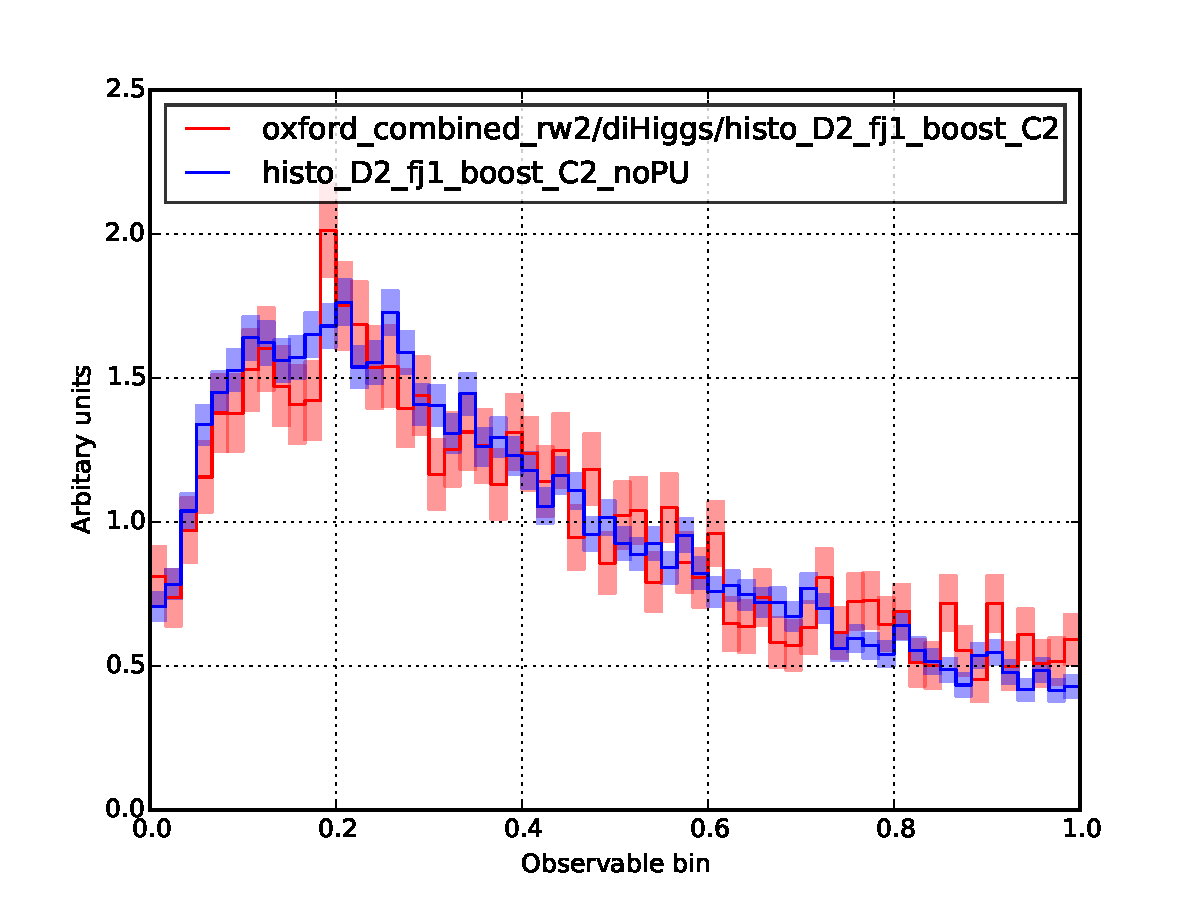
\includegraphics[width=0.60\textwidth]{plots/pu-vs-nopu-comparison-d2.pdf}
  \caption{\small
    Comparison of the distribution of the $D_2^{(\beta)}$
    substructure variable, Eq.~(\ref{eq:d2}), for the
    boosted category in two cases: without PU, and
    with $\la n_{\rm PU}\ra=150$ PU events.
    %
    In the latter case, PU has been subtracted using
    {\tt SoftKiller}.
    %
    See text for more details.
}
\label{fig: pu-vs-nopu-comparison-d2}
\end{center}
\end{figure}
%%%%%%%%%%%%%%%%%%%%%%%

\subsection{Signal significance in the presence of PU}

Finally, we revisit how the signal significance after the MVA
is affected by the inclusion of realistic PU effects.


%%%%%%%%%%%%%%%%%%%%%%%%
\begin{figure}[t]
\begin{center}
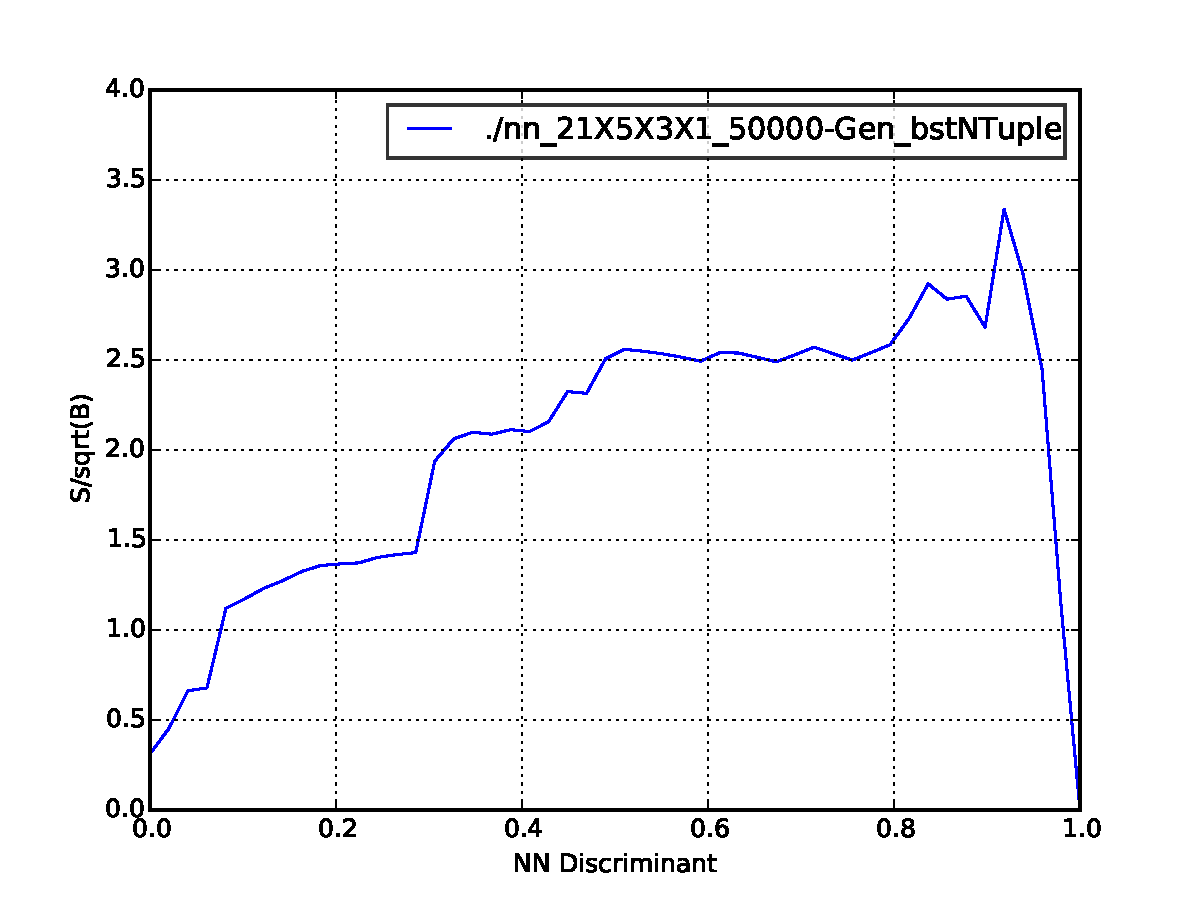
\includegraphics[width=0.48\textwidth]{plots/ssb_pu.pdf}
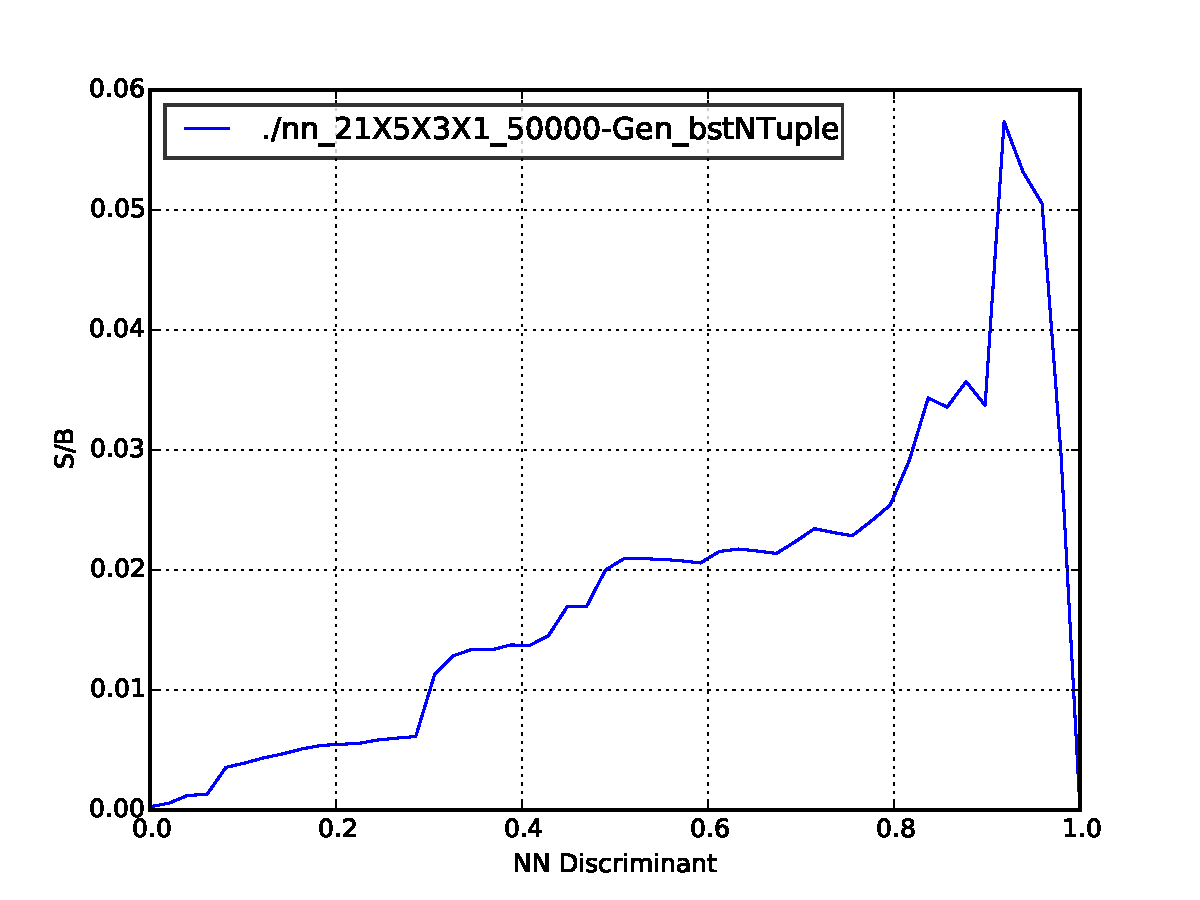
\includegraphics[width=0.48\textwidth]{plots/sb_pu.pdf}
\caption{\small
  Same as Fig.~\ref{fig:sb_mva} this time for the analysis including
  effects of PU, with $\la n_{\rm PU}\ra=150$.
}
\label{fig:sb_mva_pu}
\end{center}
\end{figure}
%%%%%%%%%%%%%%%%%%%%%%%

In Fig.~\ref{fig:sb_mva_pu} we show the signal significance,
$S/\sqrt{B}$, as well as the signal over background ratio,
$S/B$, as a function of the NN discriminant, in the case
of the analysis including the effects of PU
with $\la n_{\rm PU}\ra=150$.
%
The corresponding results in the case without PU were shown in
Fig.~\ref{fig:sb_mva}.
%
As can be seen, the MVA-driven enhancement is robust event in the
presence of PU, and a total signal significance of
almost $S/\sqrt{B}\simeq 3$ is also obtained in this case.
%
Therefore, we conclude that the qualitative results obtained
in the previous section are robust even in the presence
of realistic PU effects.
%
Note that no specific effort has been performed to
optimize PU subtraction (for example by tuning the value
of the patch length $a$ in {\tt SoftKiller}), so there is
certainly still room for improvement.
